\chapter{Cause specific mortality rates: alcohol dependence}
\label{applications-csmr}

A key assumption of the YLL estimates in GBD 2010 Study is that only
one cause leads to death.  This categorical attribution of deaths in
a mutually exclusive way has the desirable property that all assigned
deaths sum to the total number of deaths.  However, this
creates a rate that does not directly correspond to any rate in the
compartmental model (Figure \ref{forward-sim-two-compartment}) by
assuming all who die \emph{with} the condition die \emph{of} the
condition.  While this is a reasonable assumption for many conditions
such as cancer, cirrhosis or diarrhea, it is not for conditions such as
alcohol dependence, where many people die \emph{with}
the condition \emph{but not} of it.  Using alcohol dependence as an
example, this chapter compares the results of
the modeling assumptions of those who die \emph{from} alcohol dependence
and those who die \emph{with} alcohol dependence but \emph{but not} of it.

Alcohol dependence is the dysfunctional pattern of alcohol consumption
that leads to physiological dependence and impaired control.  Like
cocaine dependence in Chapter \ref{applications-splines_knot_loc}, to
be diagnosed with alcohol dependence, three or more of the seven
substance dependence criteria defined by the American Psychiatric
Association on page \pageref{page:app-substance_dependence} must be
fulfilled within a twelve-month period for a substance of alcohol.
\cite{american_psychiatric_association_diagnostic_2000, hasin_prevalence_2007}
Systematic review yielded prevalence, excess mortality and
cause-specific mortality data as seen in Figure \ref{fig:app-alcohol
  data}.

    \begin{figure}[h]
        \begin{center}
            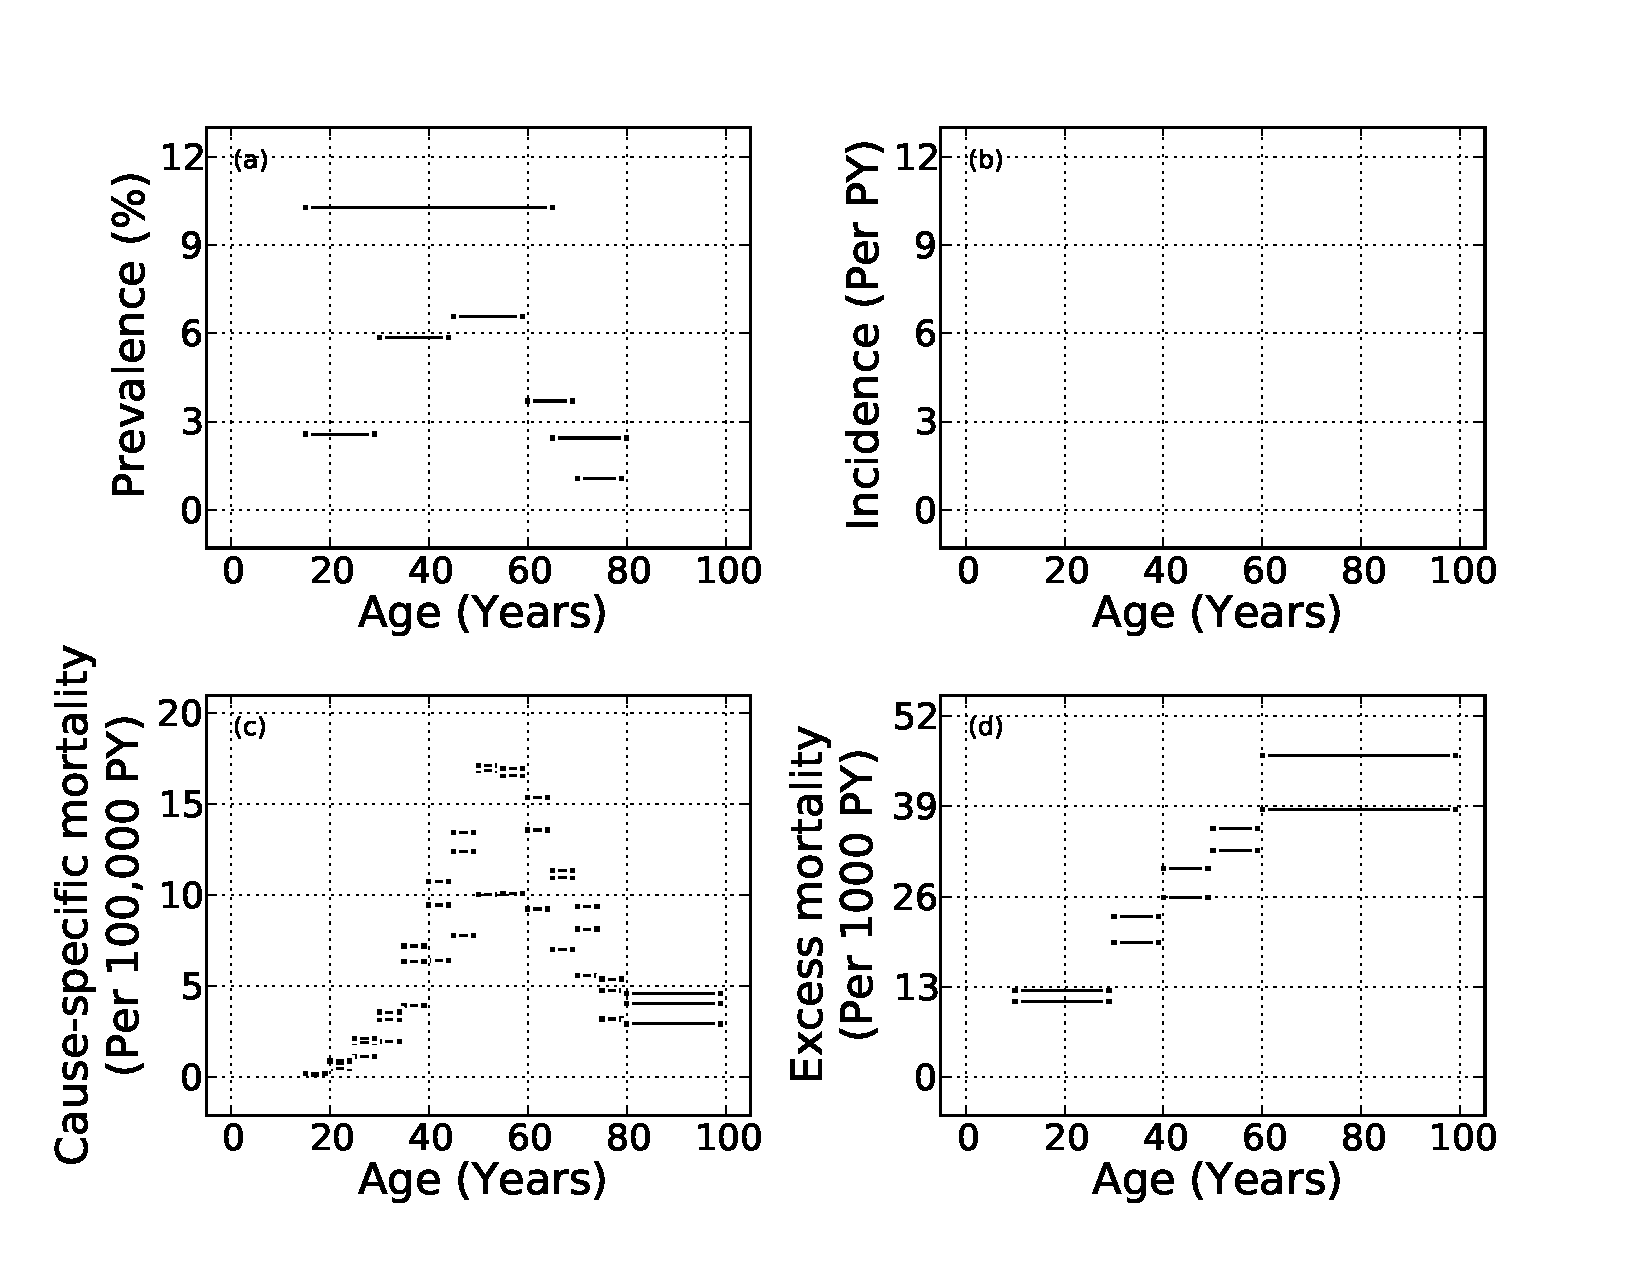
\includegraphics[width=\textwidth]{alcohol-data.pdf}
            \caption{Systematic review collected data on (a) prevalence,
              (b) incidence, (c) cause-specific mortality and (d) excess
              mortality of alcohol dependence in males from the GBD 2010
              Study region of Central Asia.}
            \label{fig:app-alcohol data}
        \end{center}
    \end{figure}

It is important to note that cause-specific mortality in this 
example means that the physician issuing a death certificate 
deemed the person died \emph{with} alcohol dependence and 
not \emph{from} alcohol dependence.  There are many reasons 
to include this data in modeling alcohol dependence.  Alcohol 
dependence has a higher mortality than recorded for two reasons.
First, alcohol use is a risk factor for many other diseases, 
including stroke and cancers.  In any individual death
from those diseases, it is not possible to determine whether alcohol
caused the death in that person.  Though at a population level, 
the higher risk associated with alcohol use can be determined.  
Second, people who drink alcohol often have other characteristics 
that lead to higher mortality risk, including tobacco smoking 
and lower socioeconomic status.

To include cause-specific mortality data in the compartmental model,
the model in Figure \ref{forward-sim-two-compartment} can be adapted
by splitting the excess mortality, $h_{f}$, into two parts (Figure
\ref{fig:two_compartment_2f})--those who die \emph{from} the
condition, $h_{f'}$, and those who die \emph{with} the condition but
\emph{not of} it, $h_{f''}$.  As described in Section
\ref{theory-csmr}, excess mortality can then be represented as the
following:
    \begin{equation}
        h_{f} = h_{f''} + h_{f'}
    \end{equation}
While the product of excess mortality and prevalence, $h_{p} \cdot h_{f}$,
can be directly measured, in practice $h_{f''}$ and $h_{f'}$ are never
disentangled.  This method implicitly separates $h_{f'}$ and $h_{f''}$
but does not try to explicitly represent both.

    \begin{figure}[h]
        \begin{center}
            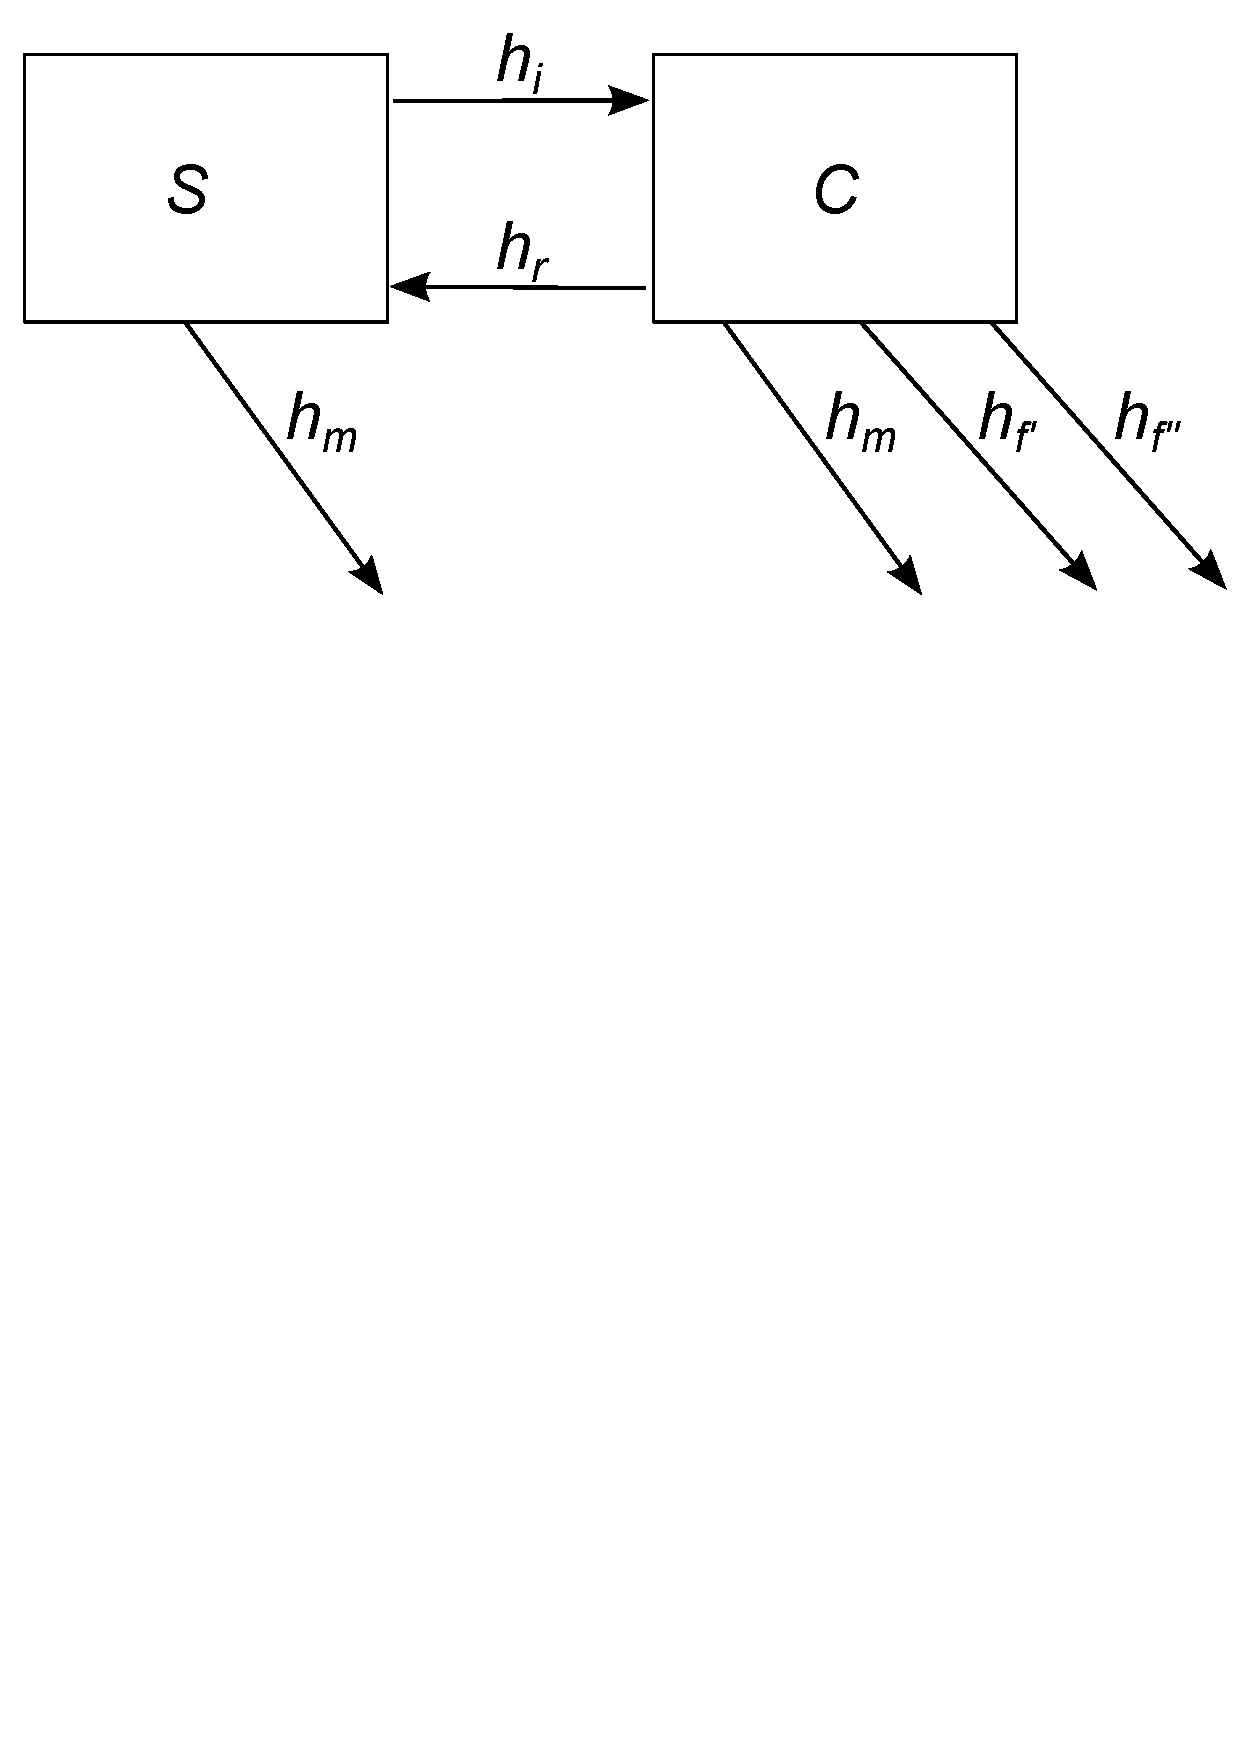
\includegraphics[width=\textwidth]{SC2.pdf}
            \caption{The two-compartment mechanistic model with the
              excess mortality split into two hazards.}
            \label{fig:two_compartment_2f}
        \end{center}
    \end{figure}

For some diseases in the GBD 2010 study, it is a reasonable assumption that
$h_{f''} = 0$, so that those who die with the condition die of it.
When this is the case, the cause-specific mortality is a direct
estimate of $h_{p} \cdot h_{f}$, a measurement of population mortality.  
However, for diseases such as alcohol
dependence, this is a poor assumption, as more die with the condition
than \emph{of} it.  When $h_{f''} \neq 0$, cause-specific mortality
data provide the lower bound of $h_{p} \cdot h_{f}$.

As seen in Figure \ref{fig:app-alcohol compare}, modeling cause-specific mortality as
$h_{f''}$ (left column, panels (a), (c) and (e)) or as $h_{f'}$ (right
column, panels (b), (d) and (f)) only change the uncertainty of the
parameter estimates and elevates the cause-specific mortality
estimates while other parameter estimates remain the same.

    \begin{figure}[h]
        \begin{center}
            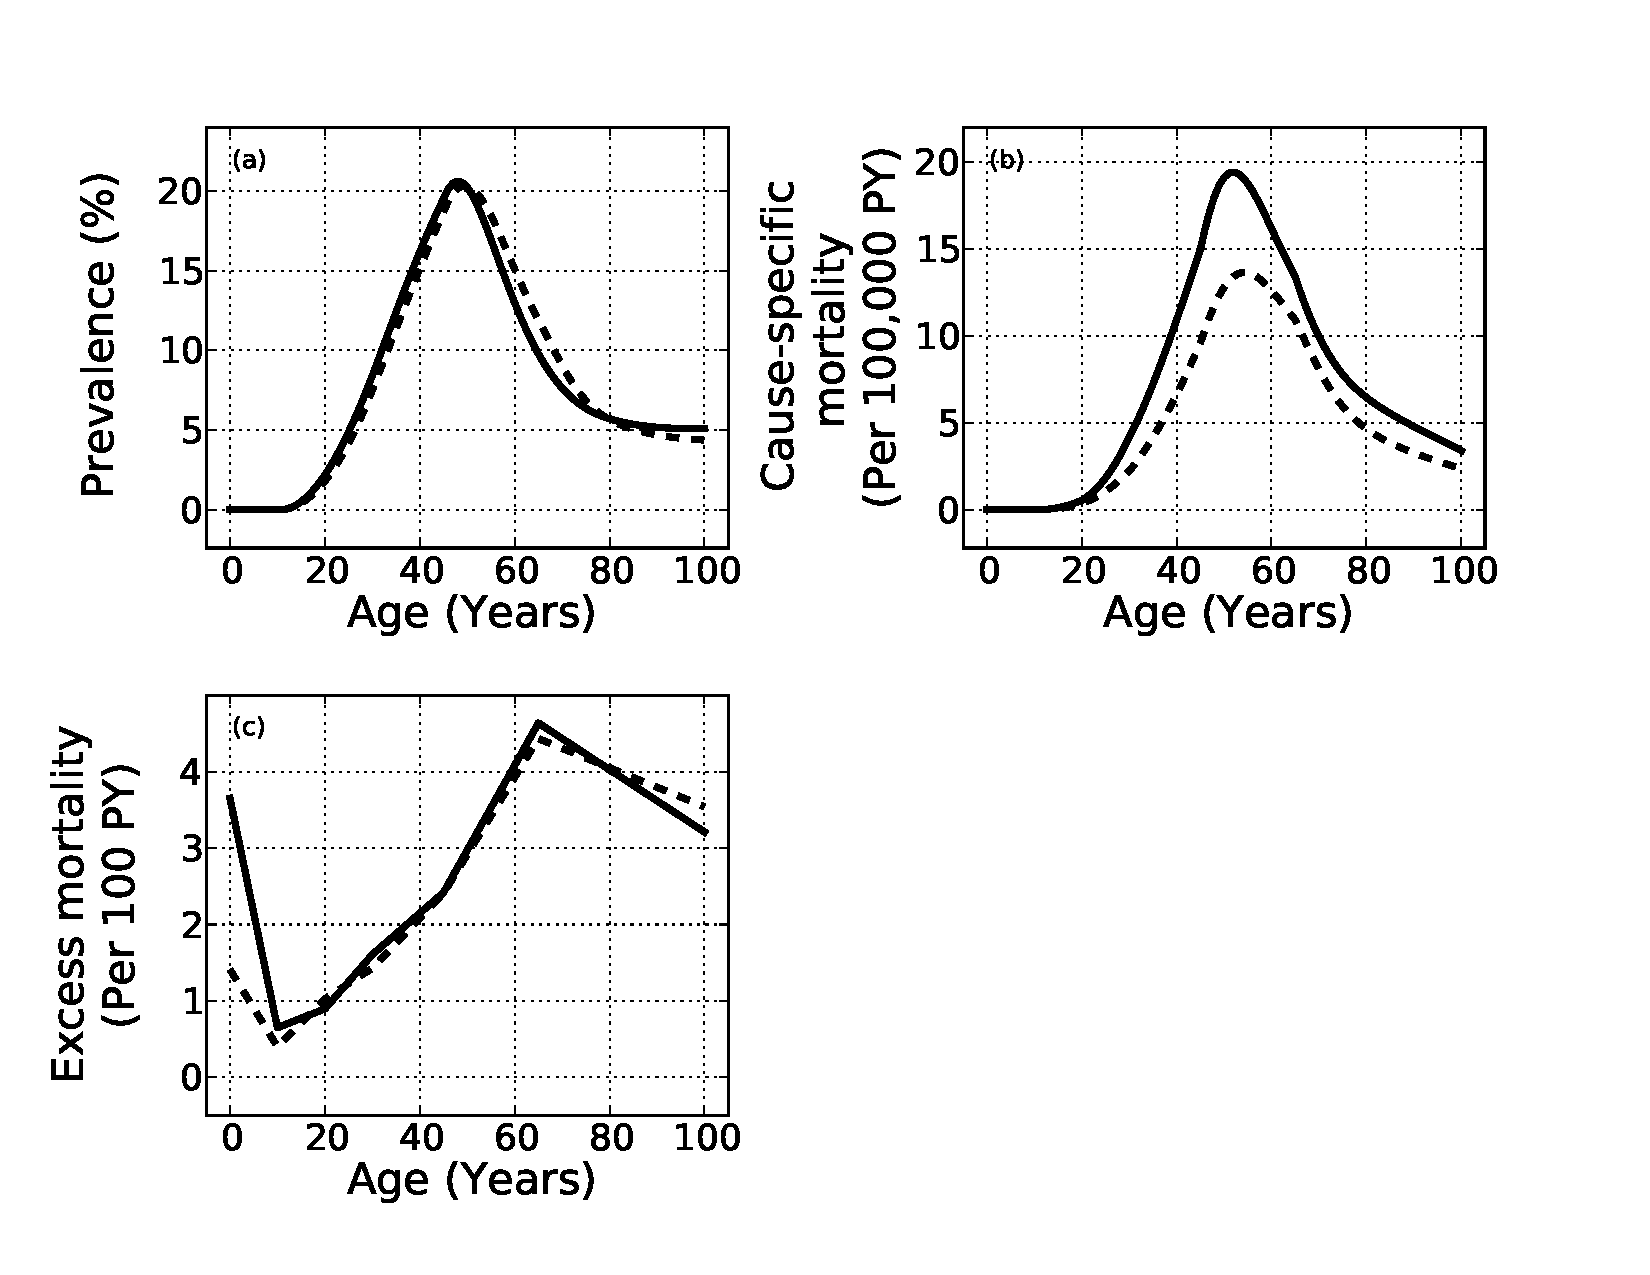
\includegraphics[width=\textwidth]{alcohol-overlay.pdf}
            \caption{Comparison of (a) prevalence,
              (b) cause-specific mortality and (c) excess
              mortality estimates of alcohol
              dependence in Central Asian males in 2005 when using
              cause-specific mortality data as a lower bound ($h_f'' \neq 0$)
              or a direct estimate of the product of
              prevalence and excess mortality ($h_f'' = 0$).}
            \label{fig:app-alcohol compare}
        \end{center}
    \end{figure}

By decomposing excess mortality into those who die from the
disease and those who die with the disease but not of the disease, the
compartmental model in Figure \ref{forward-sim-two-compartment} can
use the cause-specific mortality data as a lower bound on prevalence
times excess mortality, which is appropriate if the
disease is not exclusively coded as the underlying cause of death.
